
\documentclass[letterpaper,12pt]{article}
\usepackage[english]{babel}
\usepackage[utf8x]{inputenc}
\usepackage{amsmath}
\usepackage[paper=letterpaper,left=25mm,right=25mm,top=25mm,bottom=25mm]{geometry}
\usepackage{graphicx}
\usepackage[colorinlistoftodos]{todonotes}
\usepackage{newtxtext,newtxmath}
\usepackage{enumitem}
\usepackage{bm}

\begin{document}
	
\begin{titlepage}
	
	\newcommand{\HRule}{\rule{\linewidth}{0.5mm}}
	
	\center
	
	\textsc{\LARGE University of British Columbia}\\[1.5cm]
	\textsc{\Large MECH 325 - Mechanical Design I}\\[0.5cm]
	\textsc{\Large Assignment 2}\\[0.5cm]
	
	\HRule \\[0.8cm]
	{ \huge \bfseries Flexible Drive Design}\\[0.4cm]
	\HRule \\[1cm]
	
	{\Large GROUP C2}\\
	\vspace{0.5cm}
	
	\begin{minipage}{0.4\textwidth}
		\begin{flushleft} \large
			\emph{Team Member:}\\
			Kota Chang\\
			Chuan Du\\
			Donney Fan\\
			Dvir Hilu\\
			Michael Ko\\
			Priyansh Malik\\
			Darren Tong\\
		\end{flushleft}
	\end{minipage}
	~
	\begin{minipage}{0.4\textwidth}
		\begin{flushright} \large
			\emph{Student Number:} \\
			12345678\\
			12345678\\
			12345678\\
			12345678\\
			12345678\\
			12345678\\
			12345678
			
		\end{flushright}
	\end{minipage}\\[2cm]
	
	{\large \today}\\[2cm]
	
	{\Large\textbf{
		Performance Metric: \$ 975.49
	}}
	
	%\includegraphics{logo.png}\\[1cm]
	
	\vfill % Fill the rest of the page with whitespace
	
\end{titlepage}

\section{Summary}
\subsection{Introduction}
This document presents the design process of a roller chain drive system with bearings for the candy polishing machine, the ClumpBuster-2000. To optimize system performance and cost, we propose a 2-stage roller chain drive train connected by an intermediate shaft.

\subsection{Final Performance Results}
\begin{center}
	\begin{tabular}{ |p{3cm}||p{2cm}|p{2cm}|p{7cm}|  }
		\hline
		 & Cost (\$) & Teeth Ratio & Description \\
		\hline
		M-I Sprocket 1* &20.33 & 5.65 & 6280K553 \\
		M-I Sprocket 2 &141.83 & - & 2737T961 \\
		M-I Chain & 8.43 & - & 6261K174 \\
		I-D Sprocket 1** & 46.90 & 1.76 & 6280K233 \\
		I-D Sprocket 2 & 90.25 & - & 6236K531 \\
		I-D Chain & 22.37 & - & 6261K176 \\
		Idler Shaft &14.58 & - & 1886K61\\
		\hline
		\hline
		Lubrication & 400&- & Oil Bath Lubrication\\
		\hline
		\hline
		Maintenance & 230.8& - & Chain replacement: parts and labour\\
		\hline
		\hline
		\textbf{Total} & \textbf{975.49}& - & - \\
		\hline
	\end{tabular}
\end{center}
\noindent Note: *M-I: Motor to Intermediate Shaft, **I-D: Intermediate to Drum Shaft. Furthermore, the life of our drive train was found to be 15,000 hours, as detailed in section 2.2.5.
\subsection{Approach \& Methods}
We focused primarily on the reliability for this system while also optimizing cost. It was important for our team to ensure that our proposed design would be mechanically sound for this operation. Design decisions for the roller chain were made by following the proposed structure:
\begin{enumerate}
    \itemsep0em
    \item Identification of the \textbf{Service Classification} of the ClumpBuster-2000. In this application it was decided that the operation would fall under "Moderate Shock Load".
    \item Identification of the \textbf{Service Factor}.
    \item Determination of \textbf{Design Horsepower}.
    \item Selection of \textbf{Drive Selection}. Viable pitch chains were selected from McMaster-Carr using the calculated design horsepower and the required operational speeds.
    \item Selection of \textbf{Sprockets}. Following the recommendation in the catalogue, sprockets satisfying the design requirements for the system were found and bought from McMaster-Carr.
\end{enumerate}

\noindent The following assumptions were made in the design of the roller chain system:
\begin{itemize}
    \itemsep0em
    \item Chordal speed variations can be negligible since we are using 17 teeth sprockets.
    \item Roller chain noise level does not conflict with the requirement for minimizing the plant's ambient noise as there also exists candy polishing noise.
    \item Since the driving sprocket has 17 teeth for our design, the system will be classified under "smooth rolling" as referenced in \textbf{\textit{Martin's Sprocket Engineering Data}}. Therefore, the Service Factor ($K_s$) of each roller chain system is 1.3.
    \item Since the design horsepower at the required RPM of the system is \textbf{less} than the horsepower rating of the largest pitch chain for the desired speed, a single-strand chain drive may be used.
    \item We can machine down the shaft from 1.5 inches to 1 inch.
    \item Following Shigley's recommendation, we aimed to keep our velocity ratio below 6:1.
    \item A final speed of 120.4 rpm, a 0.33\% difference from required speed is acceptable.
    \item Adding an intermediate shaft will not change the loading conditions.
    \item We assumed roller chain efficiency to be 91\%.
\end{itemize}

\subsection{Chain System Overview}
Below is an overview diagram of the designed 2-stage roller chain drive system. One chain system transmits the torque from motor shaft to the intermediate shaft, which then has a second separate roller chain system which transmits torque from the intermediate shaft to the drum shaft. At each stage, there is a gear reduction ratio in order to reduce the 1200 RPM speed of the motor to 120 RPM which will be applied to the drum shaft.
\begin{center}
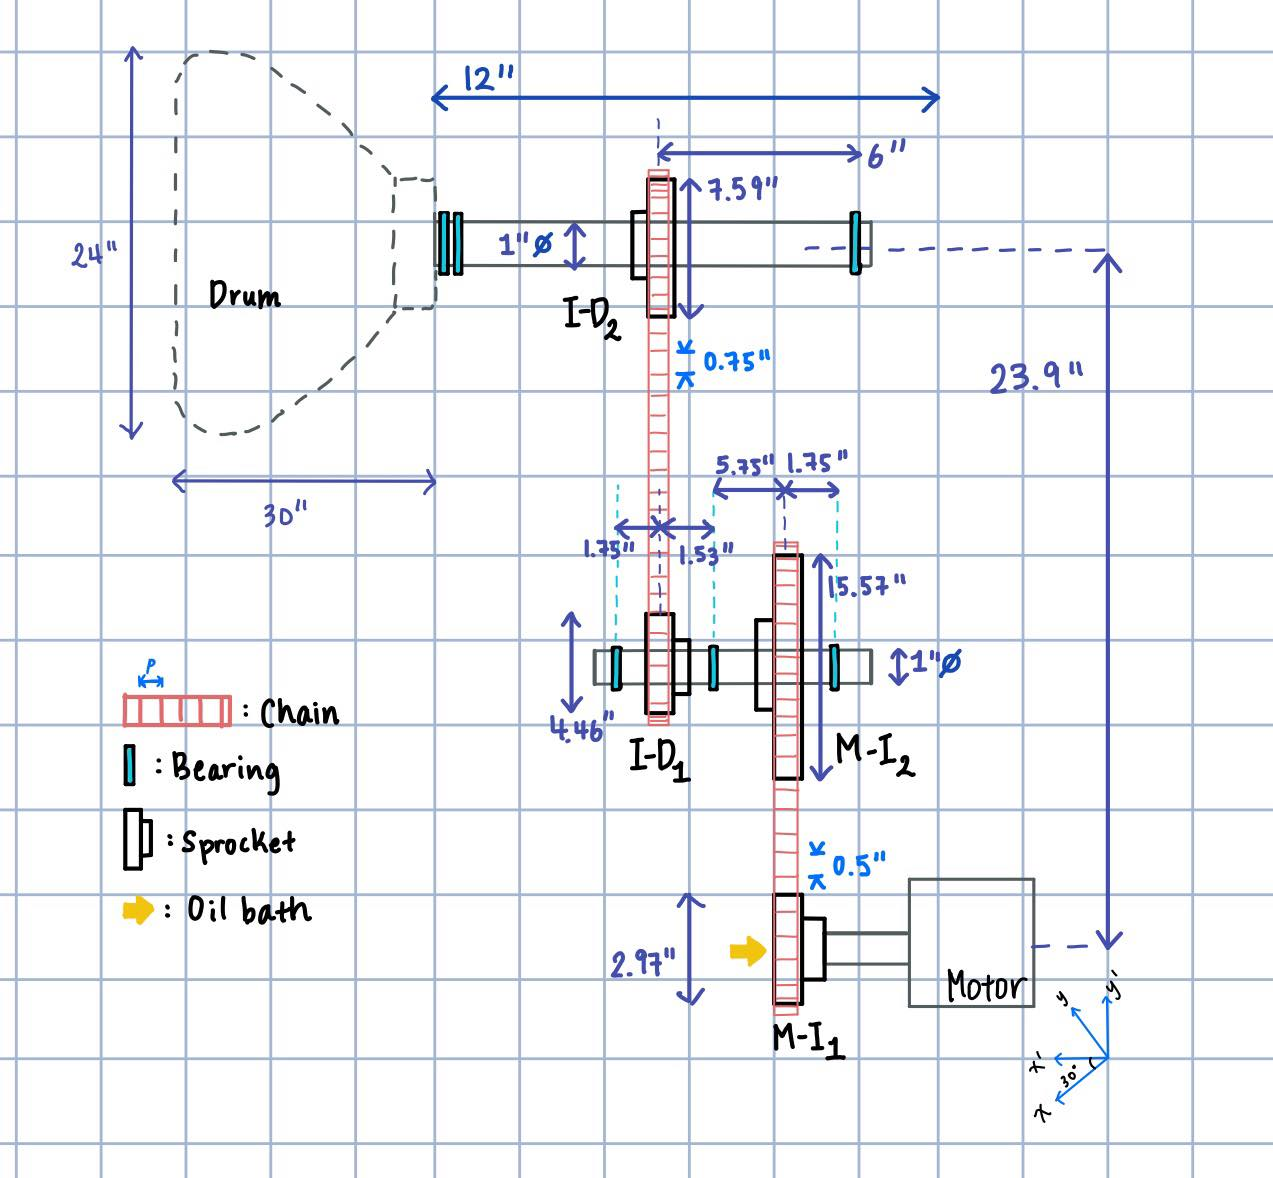
\includegraphics[width=13cm]{MECH325A2System.jpg} \\
Roller Chain, Sprocket, and Shaft Layout
\end{center}

\newpage

\section{Appendix}
\subsection{Motor Analysis}
SugarCoater-1000 operated at 30 rpm with a 40:1 reduction multi-stage gear box, therefore motor output is:
$$30 \times 40 = 1200 \text{ RPM}$$
Since the desired RPM of the shaft is 120 RPM, the reduction required is 10:1.

\subsection{Roller Chain Selection}
The guiding procedure for roller chain selection is outlined by \cite{martin}. When determining the type of chain and sprocket to use in the system, the following parameters were consider to check and justify design decisions. Throughout this analysis we will use "M-I" to indicate Motor to Intermediate Shaft drive and "I-D" for the Intermediate to Drum Shaft drive.

\subsubsection{Service Factor $\bm{K_s}$}
The service factor is identified by Table II of \cite{martin}. Due to the assumption stated in the summary that an intermediate shaft would not change loading conditions, we select the service factor $K_s$ to be 1.3.

\subsubsection{Design Power \& Factor of Safety}
The next step in the design process is validating our allowable transmitted horsepower and the safety factor. From the specification, the minimum safety factor is 2.5. We will identify our design horsepower, nominal horsepower, tabulated horsepower and then ensure we have a sufficient safety factor.
\\\\
The design horsepower is given by:
\begin{equation}
    H_d = H_{\text{nom}}K_s n_d
\end{equation}

\begin{center}
	\begin{tabular}{ |p{1.5cm}||p{1cm}|p{2cm}|p{7cm}|  }
		\hline
		Symbol & Value & Units & Description\\
		\hline
		$H_{\text{nom}}$ & 1 & hp & Nominal horsepower from motor\\
        $n_d$ & 2.5 & -  & Design Factor\\			
		$K_s$ & 1.3 & -  & Service Factor\\
		\hline
	\end{tabular}
\end{center}
Then $H_d$ = 3.25 hp. Next, we calculate the nominal horsepower:

\begin{equation}
    H_1 = 0.004 N_1^{1.08} n_1^{0.9} p^{3-0.07p}
\end{equation}

\begin{equation}
    H_2 = \frac{1000 K_r N_1^{1.5} p^{0.8}}{n_1^{1.5}}
\end{equation}

\begin{center}
	\begin{tabular}{ |p{1.5cm}||p{1.5cm}|p{1.5cm}|p{2cm}|p{7cm}|  }
		\hline
		Symbol & Chain 1 & Chain 2 & Units & Description\\
		\hline
		$N_1$ & 17 & 17 & N/A & Number of teeth in smaller sprocket\\
		$n_1$ & 1200 & 212.5 & rev/min & Sprocket speed  \\
        $p$ & 0.5 & 0.75 & in  & Chain pitch\\			
		$K_r$ & 3.4 & 17 & -  & -\\
		\hline
	\end{tabular}
\end{center}
Then we obtain:
\begin{center}
	\begin{tabular}{|p{1.5cm}|p{1.5cm}|p{1.5cm}| }
		\hline
		& Chain 1 & Chain 2\\
		\hline
		$H_1$ & 6.45 & 4.54\\
		$H_2$ & 3.29 & 305.58\\
		\hline
	\end{tabular}
\end{center}
So the tabulated horsepower $H_{\text{tab}} = \min(H_1, H_2)$ is 3.29 for Chain 1 and 4.54 for Chain 2.
\\\\
Using this tabulated horsepower, we compute the safety factor:

\begin{equation}
    H_a = H_{\text{nom}} K_s n_{fs} 
\end{equation}
where
\begin{equation}
    H_a = K_1 K_2 H_{\text{tab}}
\end{equation}
Then we find $n_{fs}$ = 2.53 for the first stage and $n_{fs}$ = 3.49 for the second, which are both greater than the minimum safety factor of 2.5. Therefore the selected sprockets satisfy the power and safety factor requirement.

\paragraph{Additional Information}
\begin{itemize}
    \itemsep0em
    \item \textbf{Nominal Power $\bm{H_{\text{nom}}}$}: This is the power as specified by the motor.
    \item $\bm{K_r}$: This is an additional factor specified by Shigley. Its value is 29 for chain numbers 25, 35; 3.4 for chain 41; and 17 for chains 40–240.
    \item \textbf{Tooth Correction Factor $\bm{K_1}$}: The value of this is 1 since the number of teeth on each driving sprocket is 17.
    \item \textbf{Multiple Strand Factor $\bm{K_2}$}: The value of this is 1 since only one strand of chain is used for each stage.
\end{itemize}

\subsubsection{Sprockets \& Lubrication}
With the design horsepower, we look at the Horsepower Tables from \cite{martin} and selected an appropriate chain pitch as well as the proper lubrication type. This table can also be found in Table 17-20 in Shigley for a 17-Tooth Sprocket.
\\\\
When choosing the sprockets, we followed these requirements:
\begin{itemize}
    \itemsep0em
    \item A minimum teeth of 17 to minimize chordal speed variation and cost.
    \item A pair of sprockets that matched the specified speed reduction.
    \item A speed reduction no greater than 6 as recommended by Shigley.
    \item A pitch that supports at least the tabulated horsepower chosen.
    \item A sufficient speed reduction in the first stage to allow for cheaper lubrication in the second.
    \item An odd number of teeth on the driving sprocket and an even number of teeth on the driven sprocket to avoid a special link.
\end{itemize}
We also note that the design horsepower was less than the horsepower rating of the largest pitch chain, so a single-strand chain was selected. With these in mind, we find a set of sprockets meeting the requirements.
\begin{center}
	\begin{tabular}{|p{4cm}|p{1.5cm}|p{1.5cm}| }
		\hline
		& M-I & I-D \\
		\hline
		Driving Sprocket Teeth & 17 & 17\\
		Driven Sprocket Teeth & 96 & 30\\
		Sprocket Pitch & 0.5 in & 0.75 in\\
		Chain Pitch No. & 41 & 60 \\
		Lubrication & Oil Bath & Manual \\
		\hline
	\end{tabular}
\end{center}

\subsubsection{Chain Length \& Center-Center Distance}
The chain length per pitch is approximated by:
\begin{equation}
\frac{L}{p} \approx \frac{2C}{p} + \frac{N_1 + N_2}{2} + \frac{(N_2 - N_1)^2}{4 \pi^2 C/p}
\end{equation}
where
\begin{equation}
    C = \frac{p}{4}\left[-A + \sqrt{A^2 - 8\left(\frac{N_2 - N_1}{2 \pi}\right)}\right]
\end{equation}
and
\begin{equation}
    A = \frac{N_1 + N_2}{2} - \frac{L}{p}
\end{equation}
\\
The procedure for choosing the chain length was as follows:
\begin{enumerate}
    \itemsep0em
    \item Estimate a reasonable center to center distance to calculate the chain length per pitch.
    \item Round the chain length per pitch to the nearest integer.
    \item Obtain a new value for the center-center distance using eqn (6).
\end{enumerate}
We obtain the following values:

\begin{center}
	\begin{tabular}{|p{4cm}|p{1.5cm}|p{1.5cm}| }
		\hline
		& M-I & I-D \\
		\hline
		Center-Center Distance & 15.57 in & 7.59 in\\
		Chain Length & 23 in & 34.5 in\\
		Price / Foot (\$/ft) & 4.4 & 7.78\\
		\hline
	\end{tabular}
\end{center}

\subsubsection{Life \& Replacement}
From Shigley Chapter 17-5, we approximate the roller chain life expectancy of 15,000 hours. The polishing machine operates 16 hours per day for 250 days per year for four years. The total operational hours is then 16,000 hours. This requires at least one chain replacement per stage, giving a maintenance cost of \$200 with an additional parts cost. Roller chains are relatively easy to replace which satisfies the maintenance requirement of the system. 

\subsection{Alternate Systems Analysis}
We analyzed both flat and V-belt flexible drive systems in addition to roller chains to assess the best design choice. This section details the reasons we moved away from the following designs. 
\subsubsection{Flat Belt Analysis}
Flat belts systems are characterized by low operating noise but also  expensive pulleys. We use the following formula to extrapolate pulley prices:
\begin{equation}
\text{Cost }=35.92 \times \text{Diameter }+17
\end{equation}

\noindent If we assume a 2-inch diameter for the small pulley, the smallest diameter we can find on McMaster-Carr is 2 inches, therefore, we need a 20 inches diameter for a 10:1 speed reduction. 
\begin{center}
	\begin{tabular}{ |p{3cm}|p{4cm}| }
		\hline
		& Price (\$) \\
		\hline
		Pulley 1 & 78.77\\
		\hline
		Pulley 2 & 735.4\\
		\hline
		Total & 814.17\\
		\hline
	\end{tabular}
\end{center}

\noindent The pulleys alone would elevate the cost of the system to \$814.17 which means if we factor in cost of belts and additional pulleys for a multi-stage system, the cost would be even higher.

\subsubsection{V-Belt Analysis}
We performed calculations for the V-Belt system and found the following parameters to be unsuitable. Given sheaves of 3 inch and 30 inch diameter, and a center-to-center distance range of 10 to 30 inches, we compute the pulley speed as follows:
\begin{equation}
    V = \pi dn/12
\end{equation}
$$V = \pi(3)(1200)/12 = 942 \text{ ft/min}$$
This is below the recommended 1000 - 5000 operating speed shown in \textbf{\textit{Shigley's Mechanical Engineering Design}} table 17-12. Consequently, we cannot design a two stage system since a single stage already decreases the belt speed to below the recommended limit. 
We compute the center-to-center distance:
\begin{equation}
    C = 0.25 \left(\left[L_p - \frac{\pi(D+d)}{2}\right]+\sqrt{\left[L_p - \frac{\pi(D+d)}{2}\right]^2-2(D-d)^2}\,\right)
\end{equation}

\begin{center}
	\begin{tabular}{ |p{1.5cm}||p{1cm}|p{2cm}|p{7cm}|  }
		\hline
		Symbol & Value & Units & Description\\
		\hline
		$LCD$ &1.8& in & length conversion factor, Table 17-11\\
		$L_p$ & 121.8 & in & Pitch length \\
        $D$ & 30 & in  & diameter of larger sheave\\			
		$d$ & 3 & in  & diameter of smaller sheave\\
		\hline
	\end{tabular}
\end{center}
We find the center-to-center distance as 32.15 inches which is higher than the 30 inches maximum allowed in the design parameters.

\subsection{Bearing Placement}
To find the most optimal location of bearing placements, namely a place where we could minimize stresses and shear forces on the shafts, torque and moments of the entire system were taken into account.

\subsubsection{Initial Torque Calculations}
We first calculate the amount of torque exerted on the shafts by the motor. This can be calculated by the following:
\begin{equation*}
    \text{Torque} = \dfrac{P}{\omega}
\end{equation*}
Where $P$ is the power supplied by the motor, and $\omega$ is the angular velocity. The total power was found using a conversion method along with assuming a 91\% efficiency rating for each roller chain system. We then obtain the following:
\begin{equation*}
    P = 745.7(0.91)^2 = 617.514 \text{ W} \\
\end{equation*}
Similarly the angular velocity was calculated by:
\begin{equation*}
    \omega = \dfrac{120 \text{ rev}}{1 \text{ min}}\dfrac{1 \text{ min}}{60 \text{ sec}}\dfrac{2\pi \text{ rad}}{1 \text{ rev}} = 12.6\, \dfrac{\text{rad}}{\text{sec}}
\end{equation*}
Then using our torque equation we obtain a final value of 49.01 Nm transferred to the drum shaft. We now work backwards through the 2-stage chain system and calculate the tension in each chain system using:
\begin{equation*}
    F_SR_S = T_S
\end{equation*}
Where $F_S$ is the tension in the roller chain, $R_S$ is the radius of the sprocket, and $T_S$ is the torque applied to the sprocket. Note that the tension in the roller chain is equal to the tangential force applied to the sprocket, which in turn is equal in magnitude to the force applied onto the shaft by the sprocket. This is such that the sprocket must stay at its location on the shaft and cannot translate along the axial direction. Applying this torque calculation we obtain the following results:
\begin{center}
	\begin{tabular}{ |p{3cm}||p{2.5cm}|p{2.5cm}|p{2.5cm}|  }
		\hline
		\multicolumn{4}{|c|}{Torque Analysis Results} \\
		\hline
		Parameter & Radius (mm) & Force (N) & Torque (Nm)\\
		\hline
		M-I Sprocket 1 & 35.27 & 142.40 & 49.01 \\
		M-I Sprocket 2 & 195.29 & 142.40 & 27.80 \\
		M-I Chain & - & 142.40 & - \\
		I-D Sprocket 1 & 52.27 & 532.12 & 27.80 \\
		I-D Sprocket 2 & 92.02 & 532.12 & 49.01 \\
		I-D Chain & - & 532.12 & - \\
		\hline
	\end{tabular}
\end{center}

\subsubsection{Placement Locations}
Using our torque calculations we are now able to find the optimal locations to place bearings on the intermediate and drum shaft (we assume we do not have to consider the motor shaft). We placed bearings such that the maximum bending moment would be minimized.\\\\
For the intermediate shaft, we first observe the following diagram:
\begin{center}
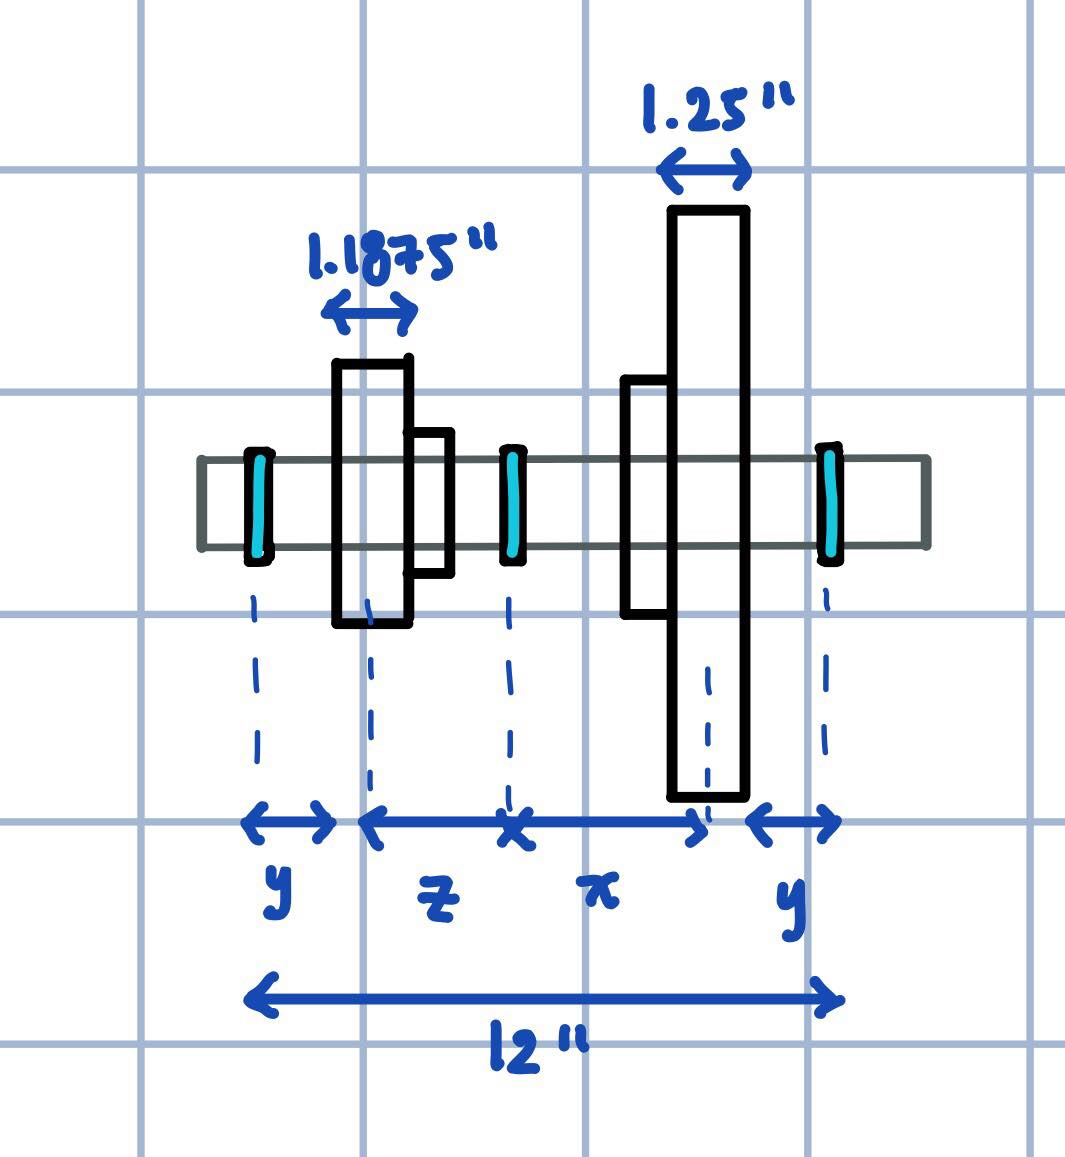
\includegraphics[width=7cm]{MECH325AIdler.jpg} \\
Intermediate Shaft Bearing Locations
\end{center}

\noindent The values of $F_1$ and $F_2$ are known, as we have already calculated them above. Note that $F_1$ is the tension force of the M-I Chain (Right Sprocket) and $F_2$ is the tension force of the I-D Chain (Left Sprocket). We then calculate the optimal positions by:
\begin{align*}
    F_1x &= F_2z \\
    F_1x &= F_2(12-x-2y-1.21875) \\
    (F_1 + F_2)x &= F_1(12-2y-1.21875) \\
    x &= \dfrac{F_1(12-2y-1.21875)}{F_1 + F_2}
\end{align*}
To minimize bending and shear, we want $x$ to be close to $y$. Graphing this we see that $y=1.75''$ gives $x=1.53''$ which is sufficiently close. We then place two bearings on the ends of the shaft and one in the position $x$ we calculated above to minimize stresses. \\\\
For the drum shaft, we observe the following diagram:
\begin{center}
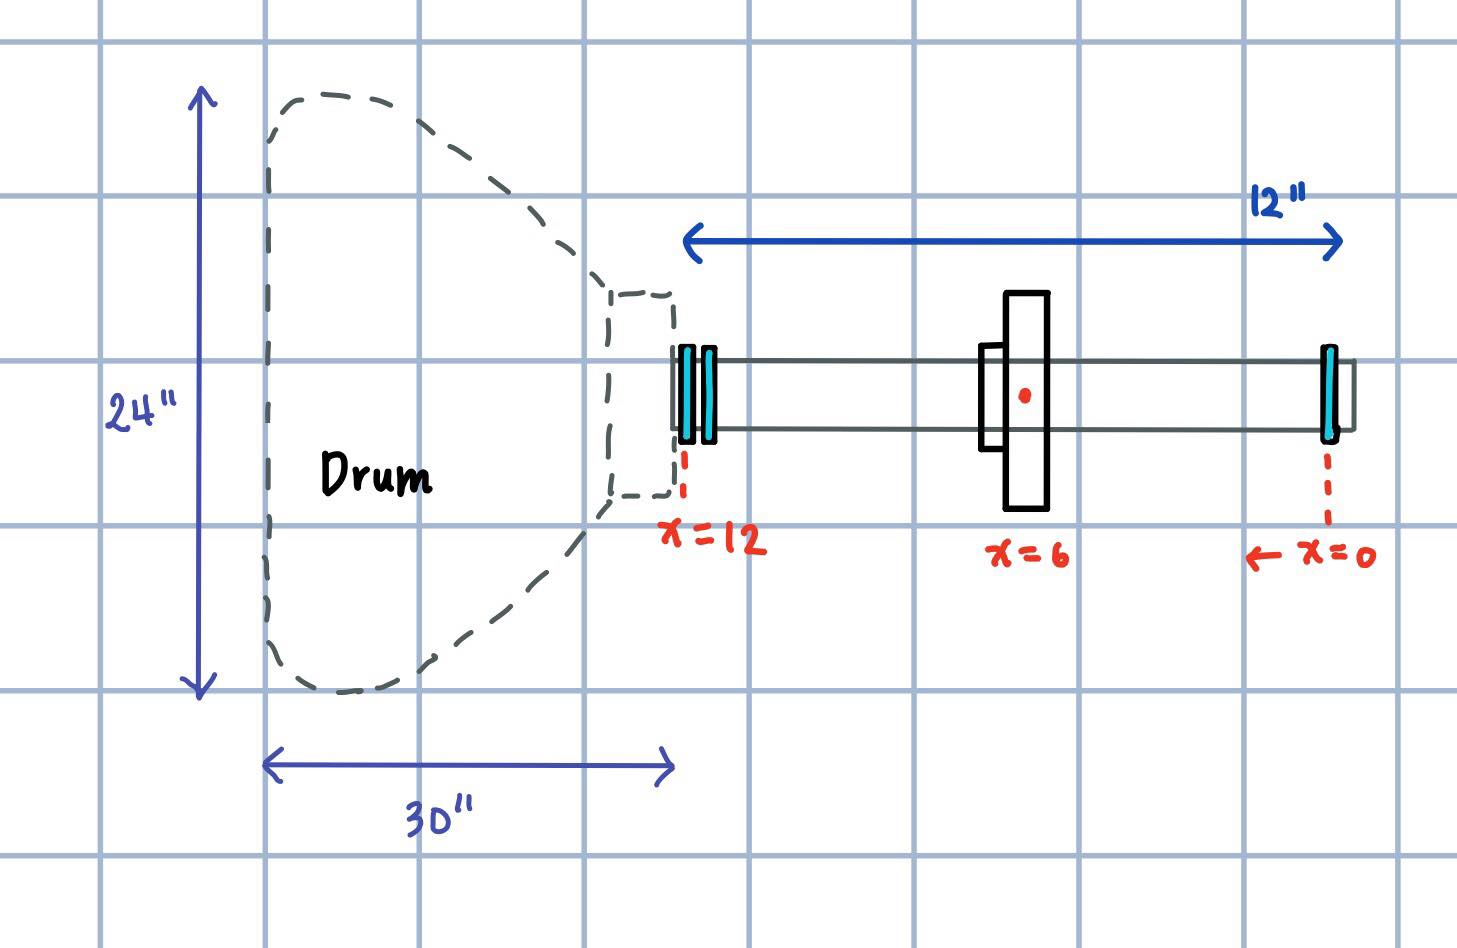
\includegraphics[width=10cm]{MECH325ADrum.jpg} \\
Drum Shaft Bearing Locations
\end{center}

\noindent We know that the ideal location to place the sprocket on this shaft would be in the middle, at $6''$ from the end as we only have one sprocket on this shaft. We then place a bearing at $x=0$ and \textbf{two} bearings on the other end. We see that there will be a load applied on this end of the shaft, which can be found by:
\begin{equation*}
    W = 150\cos(30^{\circ})
\end{equation*}
Where the load 150 lb was is the summation of the drum and candy weight and the $30^{\circ}$ comes from the orientation of the system. Therefore, we place two bearing on this end as this point would have to account for the stresses created by both the drum, candy, and sprocket loads.

\begin{thebibliography}{9}
\bibitem{shigley}
Budynas, Richard G, J K. Nisbett, and Joseph E. Shigley. Shigley's Mechanical Engineering Design. New York: McGraw-Hill, 2011. Print. 

\bibitem{martin} 
Martin Sprocket \& Gear Inc, Sprocket Engineering Data,
\\\texttt{http://www.martinsprocket.com/docs//catalogs/engineering/\\engineering\%20catalog/sprocket-engineering-data.pdf}
\end{thebibliography}

\end{document}
